%integrationstest

En test af PSoC API og SHT21p, implementeret på PCB, testes som et samlet system og dokumenteres her under.
Der anvendes et almindelig stuetermometer som referencepunkt for temperaturen. Både PSoC og SHT21p forbindes via tilslutningsprint for yderligere integration.

På figur \ref{lab:sht21p_opstilling} ses opstillingen af testen samt det anvendte termometer.
Ved første måling blev der udskrevet værdier svarende til dem som ses på figur \ref{lab:sht21p_test_resultat}, men ved yderligere målinger faldt temperaturen til omkring 5 ${^{\circ}}$C og fugtigheden steg til omkring 40 \%. 
Efter yderligere debug blev problemet lokaliseret ned til at hardwaren ikke kunne følge med softwaren, hvilket resulteret i fejlmålinger. Dette blev løst ved at indsætte et delay på 1000 ms efter at sensorens select-ben blev sat henholdsvis lav eller høj for temperatur eller fugtighed.

Ydermere var der forbundet et oscilloskop på indgangsbenet til ADCen for at måle DC-værdien fra filteret. Denne lå omkring 1,35 VDC for temperaturen og omkring 1,0 VDC for fugtighed.  


De målte DC-værdier er ved udregning omregnet til temperatur og fugtighed i ligning \ref{eq:temp_data} og ligning \ref{eq:humi_data}. Formlen herfor er opgivet i databladet for SHT21p.

\begin{equation}
temp_{pwm} = \frac{1,35}{3,3} = 0,41 
\rightarrow temp_{data} = 25,0
\label{eq:temp_data}
\end{equation}

\begin{equation}
humi_{pwn} = \frac{1,0}{3,3} = 0,30 
\rightarrow humi_{data} = 31,9
\label{eq:humi_data}
\end{equation}

\begin{figure}[htb]
  \begin{minipage}{0.48\textwidth}
    \centering
      \includegraphics[width=\textwidth]{filer/integrationstest/billeder/sht21p_opstilling}
      \caption{Opstillingen for test af SHT21p sammen med PSoC API}
    \label{lab:sht21p_opstilling}
  \end{minipage}
  \hspace{0.1\textwidth}
  \begin{minipage}{0.48\textwidth}
    \centering
      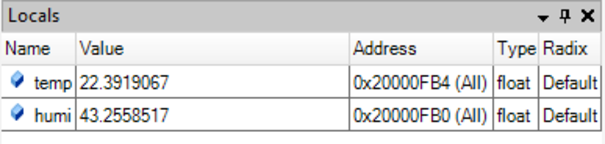
\includegraphics[width=\textwidth]{filer/integrationstest/billeder/sht21p_test_resultat}
      \caption{Måleresultater fra PSoCens debug-mode}
    \label{lab:sht21p_test_resultat}
  \end{minipage}
\end{figure}


